\documentclass[14pt, a4paper]{extarticle}
\usepackage[utf8x]{inputenc}
\usepackage[russian]{babel}
\usepackage{graphicx}
\usepackage{float}
\usepackage[outdir=./]{epstopdf}
\usepackage{booktabs}
\usepackage{tocvsec2}
\usepackage{amsfonts}
\usepackage{amsmath}
\usepackage{indentfirst}
\usepackage[left=2cm,right=2cm,bottom=3cm,top=2cm]{geometry}

\graphicspath{ {./images/} }

\linespread{1.25}

\begin{document}

\thispagestyle{empty}

\begin{center}
\ \vspace{-2.5cm}

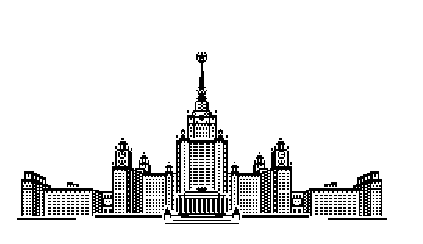
\includegraphics[width=0.5\textwidth]{msu}\\
{Московский государственный университет имени М.В. Ломоносова}\\
Факультет вычислительной математики и кибернетики\\
Кафедра автоматизации систем вычислительных комплексов

\vspace{2.5cm}

{\Large Долганов Станислав Викторович}

\vspace{1cm}

{\Large\bfseries
Метод поиска несоответствий границ объектов между результатом 2D-3D конвертации 
и используемыми картами глубины\\}

\vspace{1cm}

{\large ВЫПУСКНАЯ КВАЛИФИКАЦИОННАЯ  РАБОТА}
\end{center}

\vfill

\begin{flushright}
  \textbf{Научный руководитель:}\\
  к.ф-м.н., старший научный сотрудник\\
  Д.С. Ватолин
\end{flushright}

\vfill

\begin{center}
Москва, 2016
\end{center}

\enlargethispage{4\baselineskip}

\newpage
% Аннотация (не более полстраницы) содержит формулировку задачи и основных результатов.

\textbf{Метод поиска несоответствий границ объектов между результатом 2D-3D конвертации 
и используемыми картами глубины}

\vspace{0.5cm}
Станислав Долганов
\vspace{0.5cm}

При создании полнометражных и любительских трехмерных фильмов с помощью 
конвертации отснятого в 2D материала достаточно часто возникают дефекты, 
связанные с качеством используемых карт глубины. Такого рода артефакты, 
даже если они находятся вне салиентных регионов,  могут заметно ухудшить 
самочувствие зрителя, и, более того, вызвать головную боль. В выпускной
квалификационной работе предлагается метод поиска объектов переднего плана, границы которых 
в стереосцене не совпадают с действительностью, то есть объектов, <<слитых>> 
с фоном. Предлагаемый метод извлекает информацию о движении в сцене и 
находит несоответствия результата конвертации между извлеченным движением и глубиной сцены.
Метод был применен на 39 полнометражных фильмах, что позволило найти 125 сцен 
с заметными несоответствиями границ объектов между картой движения и картой глубины, 
использованной при конвертации.

\vspace{2cm}

\textbf{Object boundaries inconsistencies detection method 
for 2D-3D (Two-Dimensional-Three-Dimensional)
conversion results and depth maps}

\vspace{0.5cm}
Stanislav Dolganov
\vspace{0.5cm}

The creation of S3D movies by converting 2D captured footage
often introduces depth-map inaccuracies. Such artifacts can
significantly degrade the viewing experience even if they occur
only in unsalient background objects.
In this paper we propose a method for detecting foreground
objects that are stuck to the background. Our method extracts
information about motion in the scene and detects conversion-related
discrepancies between motion strength and depth. We
demonstrate the performance of the method by applying it
to 39 full-length converted 3D movies and by providing the
results of our analysis as well as examples of detected problem
shots.

\newpage
%\addcontentsline{toc}{section}{Содержание}
\tableofcontents

\newpage
\section{Введение}
% Введение должно описывать предметную область, к которой относится задача, 
% решаемая в дипломной работе, содержать неформальное ее описание.

\subsection{Стереоскопическое видео и конвертация}

В наше время практически в каждом кинотеатре мира обязательно найдется сеанс в 3D. 
Такой интерес порождает повышенный спрос на стереоконтент, однако развитие 
современных технологий производства 3D фильмов не способно в полной мере ему отвечать. 
Стандартный процесс создания контента происходит тремя возможными путями: 
\begin{itemize}
	\item съемка с помощью дорогостоящих стереоскопических систем камер,
	\item конвертация заранее отснятого двухмерного материала,
	\item использование компьютерной графики.
\end{itemize}
Последний подход относится к специфичной области мультипликационных фильмов, 
а также позволяет создавать различные спецэффекты на этапе постобработки. 
Съемка видео с помощью стереокамер требует постоянной калибровки цветовых и 
геометрических параметров камер системы, что является нетривиальным процессом и 
потому зачастую приводит к появлению некачественного контента.  Учитывая последние разработки 
в области стереоконвертации~\cite{ndjiki2011depth,tolstaya2015depth}, которые 
заметно улучшили визуальное качество результата, а также сравнительно меньшие 
затраты на производство стереофильма с помощью конвертации, 
легко заметить, что многие киностудии предпочитают конвертацию остальным подходам. 
В данном утверждении можно убедиться, если посмотреть на ежегодные соотношения 
конвертированных и отснятых фильмов за последние 60 лет~\cite{realorfake}.

\subsection{Проблемы конвертации} 

Хотя существующие программные инструменты на порядок облегчают различные 
этапы конвертации видео, сам процесс остается достаточно трудоемким и 
далеким от автоматизации. Майк Сеймор в своем обзоре~\cite{seymour2012art} 
описывает основные проблемы генерации стереовидео по исходному 2D материалу:
\begin{itemize}
	\item Эффект параллакса --- означает, что для генерации второго ракурса 
	необходимо заполнять области сцены, которые не видны на исходном ракурсе. 
	Основная проблема заключается в выборе материала для заполнения открывающихся 
	областей, который не вызывал бы дискомфорта при просмотре и был бы стабильным во времени.
	\item Эффект кулисности --- означает, что для объектов переднего плана необходимо 
	сгенерировать различную глубину для различных частей объекта, что позволит сделать 
	объект рельефным, иначе при просмотре сцены объект будет казаться плоским, 
	что противоречит реальной жизни.
	\item Эффект отжимающего действия рамки --- возникает, когда объекты с отрицательным 
	параллаксом, то есть такие объекты, которые при просмотре кажутся находящимися ближе к зрителю, 
	чем плоскость экрана, пересекают рамку экрана. Появляется невозможная в реальной 
	жизни ситуация, когда часть объекта находится перед нами, а оставшаяся часть скрыта 
	более удаленной рамкой. Наиболее точно такую ситуацию можно объяснить следующим 
	образом --- представить, что объект находится перед окном и начинает двигаться 
	от центра окна к его краю, затем часть объекта, пересекающая границу окна, пропадает.
	\item Агрессивная величина параллакса --- может проявляться различными путями. 
	Первый возможный вариант --- это большие значения как положительного, так и 
	отрицательного параллакса в сцене, что влечет за собой большой разброс объектов 
	по глубине, тяжело переносится зрителем и может стать причиной головной боли. 
	Второй вариант заключается в значительном изменении отрицательного и положительного 
	параллаксов между двумя соседними сценами. Такая ситуация требует зрителя 
	адаптироваться к каждой сцене, что также может сильно утомлять.
	\item Некачественная карта глубины. Общее качество карты глубины, которая является 
	необходимой частью процесса конвертации, прямым образом влияет на результат, 
	поэтому очень важно контролировать соответствие карты действительности, 
	что касается как верного выбора расположения объектов по глубине в сцене, 
	так и точных границ объектов.
\end{itemize}

Эффект кулисности и остальные дефекты карт глубины, которые возникают в процессе 
конвертации из 2D в 3D часто ухудшают общее восприятие зрителя от просмотра фильма. 
Наиболее значимые проблемы создают объекты, находящиеся в салиентных областях 
сцены, границы по движению которых не совпадают с границами по глубине, то есть 
таких объектов, которые движутся по пространству сцены не равномерно или деформируются, 
что невозможно в реальной жизни. Исследования в этой области~\cite{jung2012visual,li2014visual} 
подтверждают ухудшение состояния группы людей, которые смотрят такого рода стереовидео.

\subsection{Полуавтоматический контроль качества конвертации}

\begin{figure}[!h]
	\begin{minipage}[b]{1.0\linewidth}
		\centering
		\centerline{ 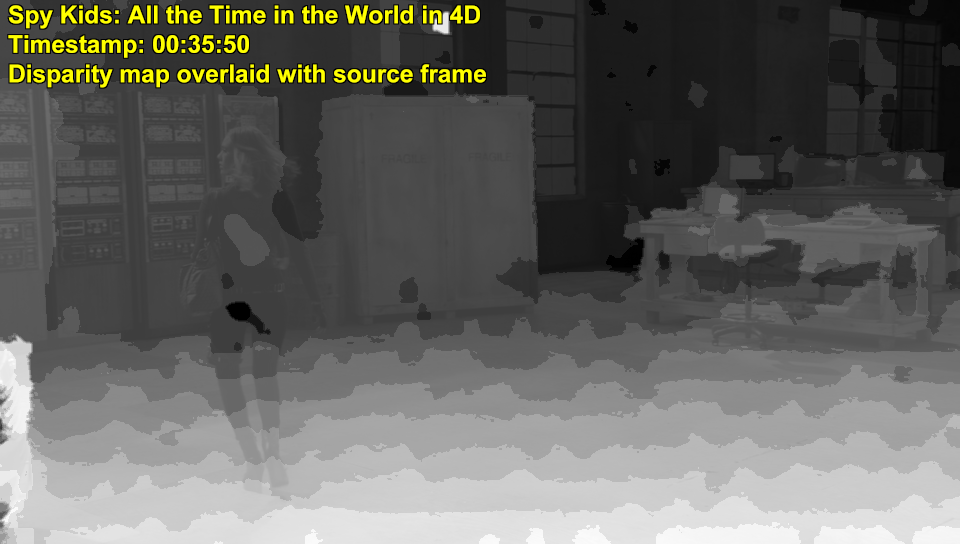
\includegraphics[width=0.7\textwidth]{example_depth} }
	\end{minipage}
	\begin{minipage}[b]{1.0\linewidth}
		\centering
		\centerline{ 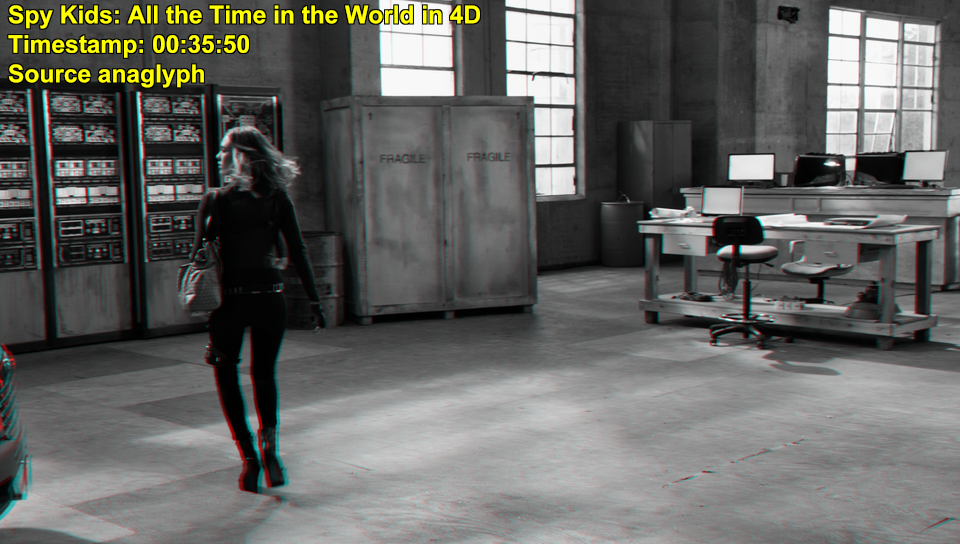
\includegraphics[width=0.7\textwidth]{example_anaglyph} }
	\end{minipage}
    \caption{Пример найденной с помощью предлагаемого метода сцены, содержащей дефект: объект переднего плана оказался слитым с фоном. Создатели фильма забыли нарисовать тело актрисы на карте глубины, поэтому сцена демонстрирует невозможную ситуацию и может вызвать визуальный дискомфорт. На верхнем изображении показана карта диспаратности поверх исходного ракурса, на нижнем --- исходная сцена в анаглифе. }
	\label{fig:example}
\end{figure}


Основной целью данной выпускной квалификационной работы 
является создание программного инструмента, 
который позволит автоматически оценить качество используемых карт глубины,
что в свою очередь позволит киностудиям создавать более качественный видеоконтент. 
Частой практикой киностудии является разделение фильма на крупные части, которые 
затем отправляются на конвертацию в специализированные компании. Такой подход 
ухудшает качество, так как компании не знают о результатах работы друг друга. 
Основной выигрыш для киностудии --- это уменьшение времени, которое понадобиться 
для конвертации, однако из-за сжатых сроков, а так же ручного тестирования 
качества результата, часто возникают такие сцены, как на Рис.~\ref{fig:example}. 
Предлагаемый программный инструмент позволит проводить проверку в полуавтоматическом 
режиме, что несомненно повысит как качество, так и время производства.
В качестве входных данных предлагаемому алгоритму требуются стереовидеопоследовательность 
и опционально карты глубины, используемые во время конвертации в 3D формат данной 
видеопоследовательности. В случаях, когда информация об используемых картах 
глубины недоступна, метод оценивает карту диспаратности с помощью~\cite{simonyan2008fast,zhang2014100+}. 
Он находит дефекты, сравнивая для каждого отдельного 
кадра границы карты глубины/диспаратности с границами карты 
амплитуды движения. Такой подход позволяет находить движущиеся объекты, которые 
частично или полностью отсутствуют на оцениваемой карте глубины. Так как не существует 
общепринятого быстрого и качественного алгоритма оценки векторов движения, было принято 
решение использовать в качестве такого алгоритма~\cite{simonyan2008fast}, который 
применяется к последовательности левых ракурсов. Затем полученная последовательность 
оценненых карт амплитуды движения итеративно улучшается с помощью временных и 
пространнственных фильтраций~\cite{fecker2007time,matyunin2011temporal,he2013guided}. 
Результирующая оценка для каждого кадра высчитывается, как величина несоответствия 
глубины и движения. Оценка для сцены высчитывается, как средневзвешенная оценка 
соответствующих кадров, где веса высчитываются на основании доверия 
к оцененными векторам движения.

\newpage
\section{Постановка задачи}
% Постановка задачи должна содержать формулировку задачи в рамках определенной модели 
% предметной области, к которой относится решаемая задача, требования к искомому решению 
% в терминах используемой модели предметной области.

\subsection{Неформальная постановка задачи}

Пусть имеются две видеопоследовательности, одна из которых снята на камеру, 
а вторая получена с помощью конвертации таким образом, 
что видеопоследовательности вместе являтся ракурсами стереоскопического видео. 
Также опционально может иметься видеопоследовательность, состоящая из карт глубины, 
использованных для конвертации. Требуется определить наличие объектов, <<слитых>> с фоном, 
то есть объектов, границы которых по глубине не совпадают с действительностью.

\subsection{Формальная постановка задачи}

Обозначения:

\textit{Пиксель} $p$ --- тройка $<p_r,p_g,p_b>$ целых чисел от 0 до 255, 
определяющих цветовые компоненты в пространстве RGB.

\textit{Изображение} $I$ --- матрица размера $h \times w$ из пикселей.

\textit{Видеопоследовательность} $\{I_t\}_{t=0}^N$ --- конечный упорядоченный набор 
изображений (кадров) одинаковых размеров.

\begin{figure}[!h]
	\begin{minipage}[b]{1.0\linewidth}
		\centering
		\centerline{ 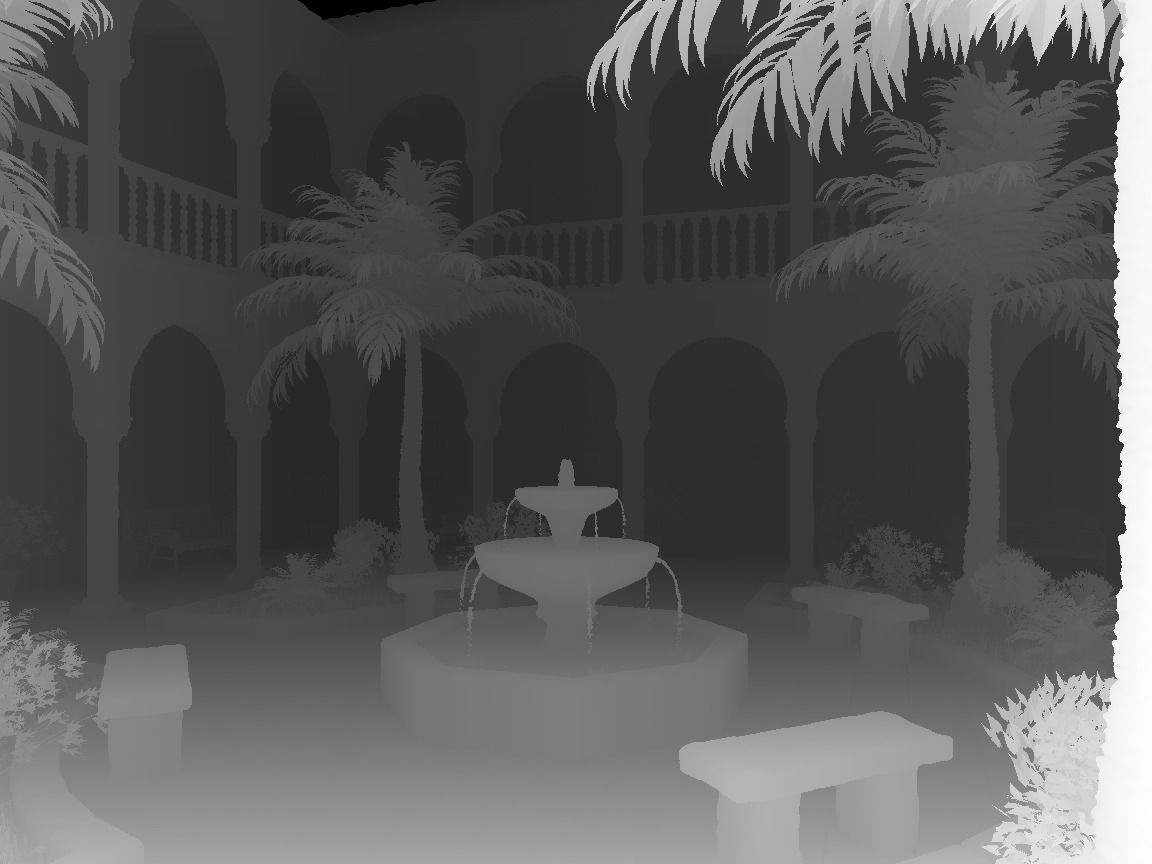
\includegraphics[width=0.7\textwidth]{depth_map_example} }
	\end{minipage}
    \caption{Пример карты глубины.}
	\label{fig:depth_map_example}
\end{figure}


\textit{Карта глубины} $D$ --- матрица размера $h \times w$, состоящая из чисел от 0 до 255,
определяющая расстояние от позиции смотрящего до всех объектов в сцене, 
где значение 255 соответствует положению смотрящего, 128 плоскости экрана, 
а 0 --- <<бесконечности>>. Пример Рис.~\ref{fig:depth_map_example}.

\textit{Последовательность карт глубины} $\{D_t\}_{t=0}^N$ --- конечный упорядоченный 
набор карт глубины одинаковых размеров, которые используются алгоритмом конвертации 
для извлечения информации о расположении объектов в сцене.

\textit{Конвертированное стереовидео} $S$ --- упорядоченная пара видеопоследовательностей 
($\{L_t\}_{t=0}^N$,$\{R_t\}_{t=0}^N$), совпадающих по количеству и размеру кадров, 
где $\{L_t\}_{t=0}^N$ --- это снятая видеопоследовательность, а $\{R_t\}_{t=0}^N$ --- 
полученная на основании $\{L_t\}_{t=0}^N$ и $\{D_t\}_{t=0}^N$, конвертированная последовательность. 
Видеопоследовательности называются левым и правым ракурсом соответственно.

\textit{Оценка} $q$ --- действительное неотрицательное число $q \in \mathbb{R}^{+} \cup \{0\}$, 
пропорциональное величине заметности артефакта в стереопаре.

Постановка задачи:

\begin{enumerate}
	\item На вход алгоритму, реализующему разрабатываемый метод, 
	подаётся конвертированное стереовидео $S$, а также дополнительно может быть 
	передана последовательность карт глубины $\{D_t\}_{t=0}^N$.
	\item Выходом алгоритма является набор оценок $\{q_t\}_{t=0}^N$, 
	соответствующих кадрам входящей стереовидеопоследовательности.
\end{enumerate}

\subsection{Требования к методу}

Разрабатываемый метод должен быть применим для анализа полнометражных 
стереоскопических фильмов. Соответственно, он должен удовлетворять следующим требованиям:

\begin{itemize}
	\item Способность находить сцены с заметными артефактами, 
	находящимися в областях салиентного движения.
	\item Низкая доля ошибок первого рода (пропуск сцены) при приемлемой доле 
	ошибок второго рода (ложное срабатывание). Ошибки второго рода менее существенны, 
	так как если ложных срабатываний не очень много, их можно исключить 
	при ручном просмотре обнаруженных сцен.
	\item Высокая скорость работы на видеопоследовательностях высокого разрешения 
	вплоть до $1920 \times 1080$. Требуется для того, чтобы анализ 
	полнометражного стереоскопического фильма занимал приемлемое время.
	\item Устойчивость к другим типам артефактов, главным из которых является отсутствие 
	глубины в сцене (сцена выглядит плоской, либо присутствует только некоторый градиент по глубине).
\end{itemize}

\subsection{Цели выпускной квалификационной работы}

Целью выпускной квалификационной работы является разработка метода, решающего поставленную задачу 
с минимальной долей ошибок первого рода (артефакт не обнаружен) и 
с приемлемой долей ошибок второго рода (ложное срабатывание).

В рамках выпускной квалификационной работы предполагается решить следующие задачи:

\begin{enumerate}
	\item Провести обзор предметной области алгоритмов оценки качества конвертированного стереовидео.
	\item Разработать метод поиска несоответствий границ объектов между результатом 2D-3D конвертации 
	и используемыми картами глубины, учитывая требования данной задачи.
	\item Разработать алгоритм, реализующий метод, и провести его экспериментальную оценку 
	на соответствие требованиям решаемой задачи.
	\item Произвести массовый анализ реальных стереоскопических фильмов 
	на предмет наличия движущихся объектов, слитых с фоном.
\end{enumerate}


\newpage
\section{Обзор предметной области}
% Обзор должен содержать явно сформулированные цели и критерии сравнения, которые 
% должны коррелировать с требованиями к искомому решению исходной задачи. 
% В конце обзора должны быть сформулированы выводы.

\subsection{Методы оценки качества 2D видеопоследовательностей}

Многие годы ислледователи изучали качество 2D видеопоследовательностей. 
Wang~\cite{wang2006survey} предложил исчерпывающий обзор основных подходов в данной области.
Самым популярным методом является \textbf{Peak-Signal-to-Noise-Ratio (PSNR)}:
\begin{equation*}
	MSE = \frac{\sum_{i=0}^{h}\sum_{j=0}^{w}[I(i, j) - I'(i, j)]^2}{h \cdot w},
\end{equation*}
\begin{equation}
	PSNR = 20 \cdot \log_{10}(\frac{255}{MSE}),
\end{equation}
где $I$, $I'$ два изображения, которые сравниваются. Чем выше значение $PSNR$, 
тем больше похожи изображения, $PSNR \equiv +\infty$ соответствует одинаковым изображениям. 
Метод \textbf{Structural Similarity Index (SSIM)} многими исследователями был принят, 
как основной метод оценки качества, приближающий субъективную оценку. Данный метод встречается
практически в каждой статье и описывается следующим уравнением:
\begin{equation}
	SSIM = \frac{(2\bar{x}\bar{y} + C_1)(2\sigma_{xy} + C_	2)}{[\bar{x}^2 + \bar{y}^2 + C_1](\sigma_x^2 + \sigma_y^2 + C_2)},
\end{equation} 
где $\bar{x}$, $\bar{y}$, $\sigma_x$, $\sigma_y$, $\sigma_{xy}$ --- среднее значение 
для первого изображения, среднее значение для второго изображения, дисперсия для $x$, 
дисперсия для $y$, ковариация $x$ и $y$; $C_1$, $C_2$ --- константы. Значение $SSIM$ 
высчитывается с помощью скользящего окна размером $11 \times 11$ с весами Гауссового ядра, 
а итоговое значение для двух изображений --- это среднее по всем насчитанным окнам.

\subsection{Методы оценки качества стереоскопического видео}

Основными направлениями исследований в области оценки качества стереоскопического видео 
являются множественные несоответствия между ракурсами и временная стабильность 
динамического диапазона глубины. Voronov в соавторстве~\cite{voronov2012towards} предложил
способ нахождения разницы между ракурсами по цвету, резкости, 
а также различных геометрических искажений. В статье~\cite{akimov2012automatic} авторами 
был предложен метод нахождения перепутанных ракурсов в стереовидео. 

Артефакты, влияющие на качество конвертированного стереоскопического видео, более 
разнообразны и менее изучены в научных кругах. Bokov в соавторстве~\cite{bokov2014automatic} 
предложил алгоритм поиска трех основных проблем, возникающих при конвертации:
\begin{itemize}
	\item Резкость границ объектов,
	\item Эффект кулисности,
	\item Плоские сцены.
\end{itemize}
Ожидаемо, данный алгоритм подходит для обнаружения проблем только для тех объектов, 
которые присутствуют на карте глубины. В данной выпускной
квалификационной работе предлагается 
дополнительный метод, расширяющий возможности оценки качества конвертированного стереовидео,
позволяющий находить объекты переднего плана, частично или полностью отсутствующие
на используемых картах глубины.

\subsection{Обзор базовых алгоритмов}

Предлагаемый метод является композицией двух крупных областей исследований: извлечение структуры 
сцены на основании информации о движении, а также алгоритмов сопоставления краев и контуров 
между двумя картами границ. Обе области достаточно хорошо изучены.

Многие методы извлечения структуры сцены из движения предполагают минимизацию функции энергии
с членом, отвечающим амплитуде движения, извлеченной из сцены. Яркий 
представитель~\cite{zhang2009consistent} дополнительно учитывает ограничение, 
обеспечивающее временную стабильность, а также уточняет положение объектов с помощью ротации 
в пространстве плоскостей, соответствующих цветовым сегментам кадра, в сторону уменьшения энергии.
Такой подход позволяет извлекать карты глубины высокого качества, обладающие временной стабильностью.
Однако временная сложность алгоритма не подходит для решения прикладных задач, в частности 
для анализа полнометражного стереоскопического фильма. Недавно предложенный метод
фильтрации~\cite{he2013guided}, сохраняющий края объектов, позволил положить в основу разрабатываемого
метода менее вычислительно сложный подход: изначально извлекается сырая карта амплитуды движения 
с помощью блочного алгоритма оценки векторов движения~\cite{simonyan2008fast}, а затем улучшается
путем свертки фильтром, сохраняющим границы объектов.

Для решения задачи сопоставления контуров, было рассмотрено несколько современных точных алгоритмов
сопоставления замкнутых контуров. Например, Xu в соавторстве~\cite{xu20092d} предложил метод,
основанный на дексрипторе гибкости контуров. Расширение на случай не замкнутых контуров возможно, 
однако потребует использования не самого точного алгоритма водоразделов~\cite{roerdink2000watershed}, 
что повлечет значительное увеличение ошибок второго рода. Другой 
подход~\cite{felzenszwalb2007hierarchical} заключается в использовании особой структуры ---
иерархического дерева форм. К сожалению, данный метод не расширяется на разрывные контура, 
что критично в нашем случае, так как оценка карт амплитуды движения не является идеальной и содержит
в том числе большое количество контуров, не являющихся непрерывными и замкнутыми. Таким образом, 
в ходе анализа предметной области было решено использовать менее точный, но более устойчивый
к качеству анализируемых контуров метод, схожий с distance transform~\cite{borgefors1986distance}.

\subsection{Выводы}

В ходе обзора предметной области были сделаны следующие выводы о структуре проектируемого метода:

\begin{itemize}
	\item Использовать блочный алгоритм оценки векторов движения с последующим улучшением
	путем свертки фильтром, сохраняющим границы объектов. Такой подход не даст самой высокой 
	точности, однако позволит провести анализ за разумное время.
	\item Использовать похожий на distance transform алгоритм сопоставления контуров, устойчивый
	к входным данным, потенциально поврежденным, как следствие неидеальности используемых методов.
\end{itemize}

\newpage
\section{Предложенный метод}

\subsection{Краткое описание метода}

\begin{figure}[!h]
	\begin{minipage}[b]{1.0\linewidth}
		\centering
		\centerline{ 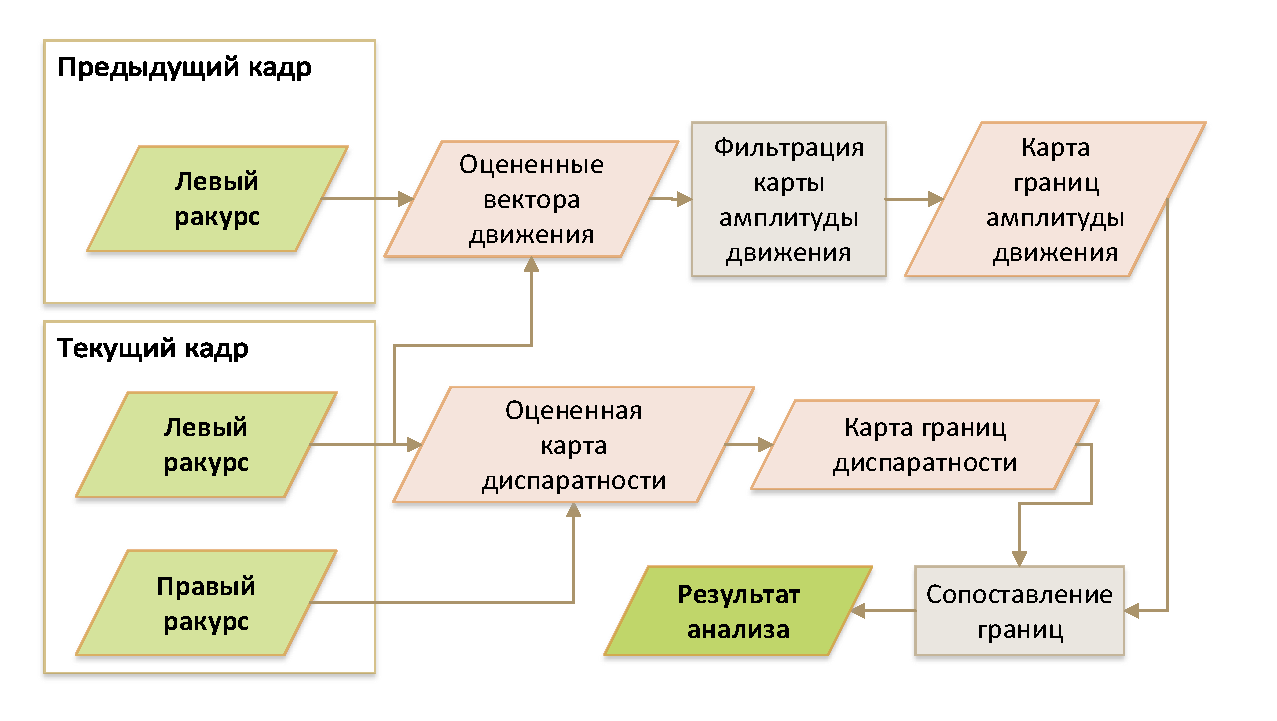
\includegraphics[width=\textwidth]{full_pipeline_rus.pdf} }
	\end{minipage}
    \caption{ Схема предлагаемого метода. Шаг оценки карты диспаратности 
    	может быть опущен в случае, когда доступна оригинальная карта глубины. }
	\label{fig:full}
\end{figure}


На Рис.~\ref{fig:full} изображена схема предлагаемого метода поиска несоответствий между
движением объекта и картой глубины, используемой во время конвертации видео из 2D в 3D.
Входными данными метода являются стереоскопическое видео, конвертированное из 2D, и,
опционально, карта глубины, участвующая в процессе конвертации. Результатом работы
алгоритма, реализующего метод, является покадровая оценка, которую можно интерпретировать 
как периметр объектов, отсутствующих на карте глубины. Метод состоит из следующих шагов:

\begin{enumerate}
	\item Оценить вектора движения левого ракурса между предыдущим и текущим кадром.
	\item Оценить карту диспаратности между левым и правым ракурсом (в случае недоступности карты глубины).
	Использование карты диспаратности вместо карты глубины допустимо, так как методу требуется
	знание только о границах объектов по глубине, которые совпадают с границами на карте диспаратности.
	\item Рассчитать карты амплитуды движения, используя поле векторов движения, улучшенное
	с помощью временной и пространственной фильтрации для достижения временной целостности.
	\item Провести сопоставление границ между картами амплитуды движения и глубины.
	\item Рассчитать площадь границ карты амплитуды движения, которые отсутствуют на карте глубины.
	Эта площадь и будет являться финальной оценкой.
\end{enumerate}

\subsection{Карта амплитуды движения}

\begin{figure}[!h]
	\begin{minipage}[b]{1.0\linewidth}
		\centering
		\centerline{ 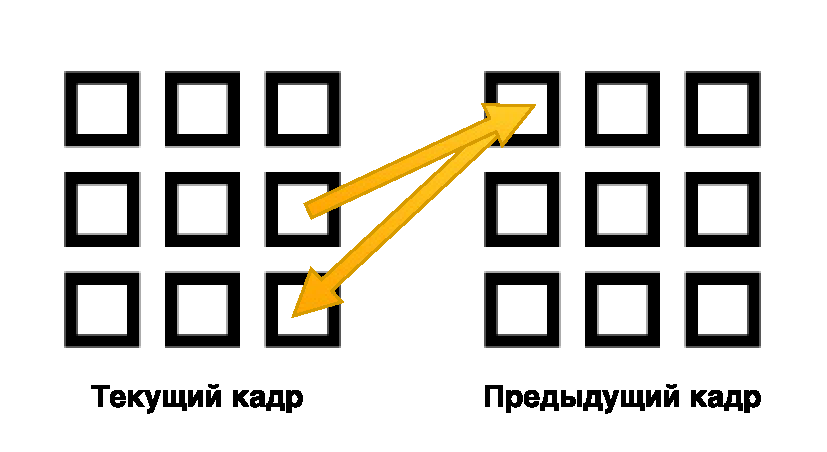
\includegraphics[width=0.7\textwidth]{lrc} }
	\end{minipage}
    \caption{Пример ситуации, когда пиксели при проверке значения LRC не совпадают. }
	\label{fig:lrc}
\end{figure}


Для извлечения как карты движения, так и карты диспаратности, применяется блочный подход,
описанный в~\cite{simonyan2008fast}. Для оценки значения доверия к получившимся картам используется
ограничение left\slash right-consistency (LRC)~\cite{egnal2004stereo} (которое, в случае оценки движения,
означает разницу между исходным пикселем и пикселем после перехода по вектору движения 
вперед и назад по вектору, построенному из прошлого в текущий кадр Рис.~\ref{fig:lrc}).

\begin{figure}[!h]
	\begin{minipage}[b]{0.49\linewidth}
		\centering
		\centerline{ 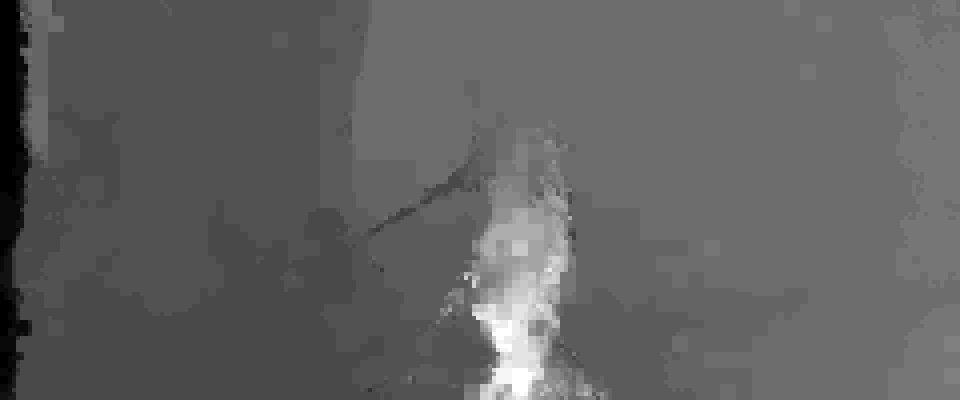
\includegraphics[width=\linewidth]{motionx} }
		\centerline{\scriptsize{(a) Horizontal-motion strength map}}\medskip
	\end{minipage}%
	\hfill
	\begin{minipage}[b]{0.49\linewidth}
		\centering
		\centerline{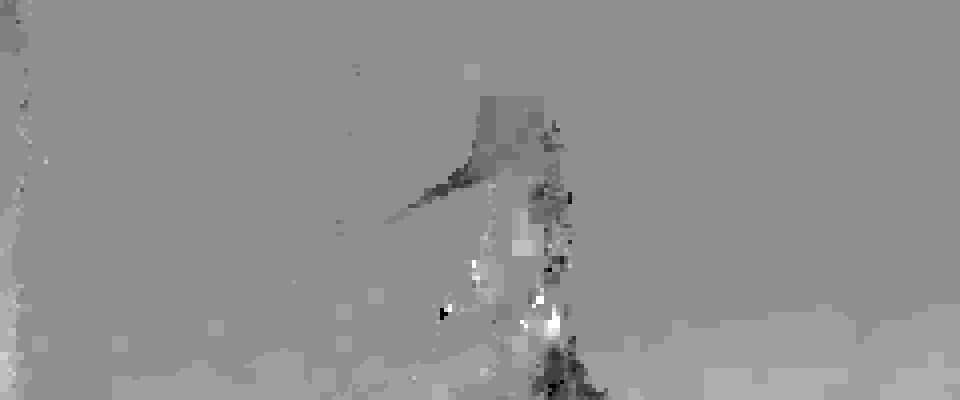
\includegraphics[width=\linewidth]{motiony} }
		\centerline{\scriptsize{(b) Vertical-motion strength map}}\medskip
	\end{minipage}
	\begin{minipage}[b]{0.49\linewidth}
		\centering
		\centerline{ 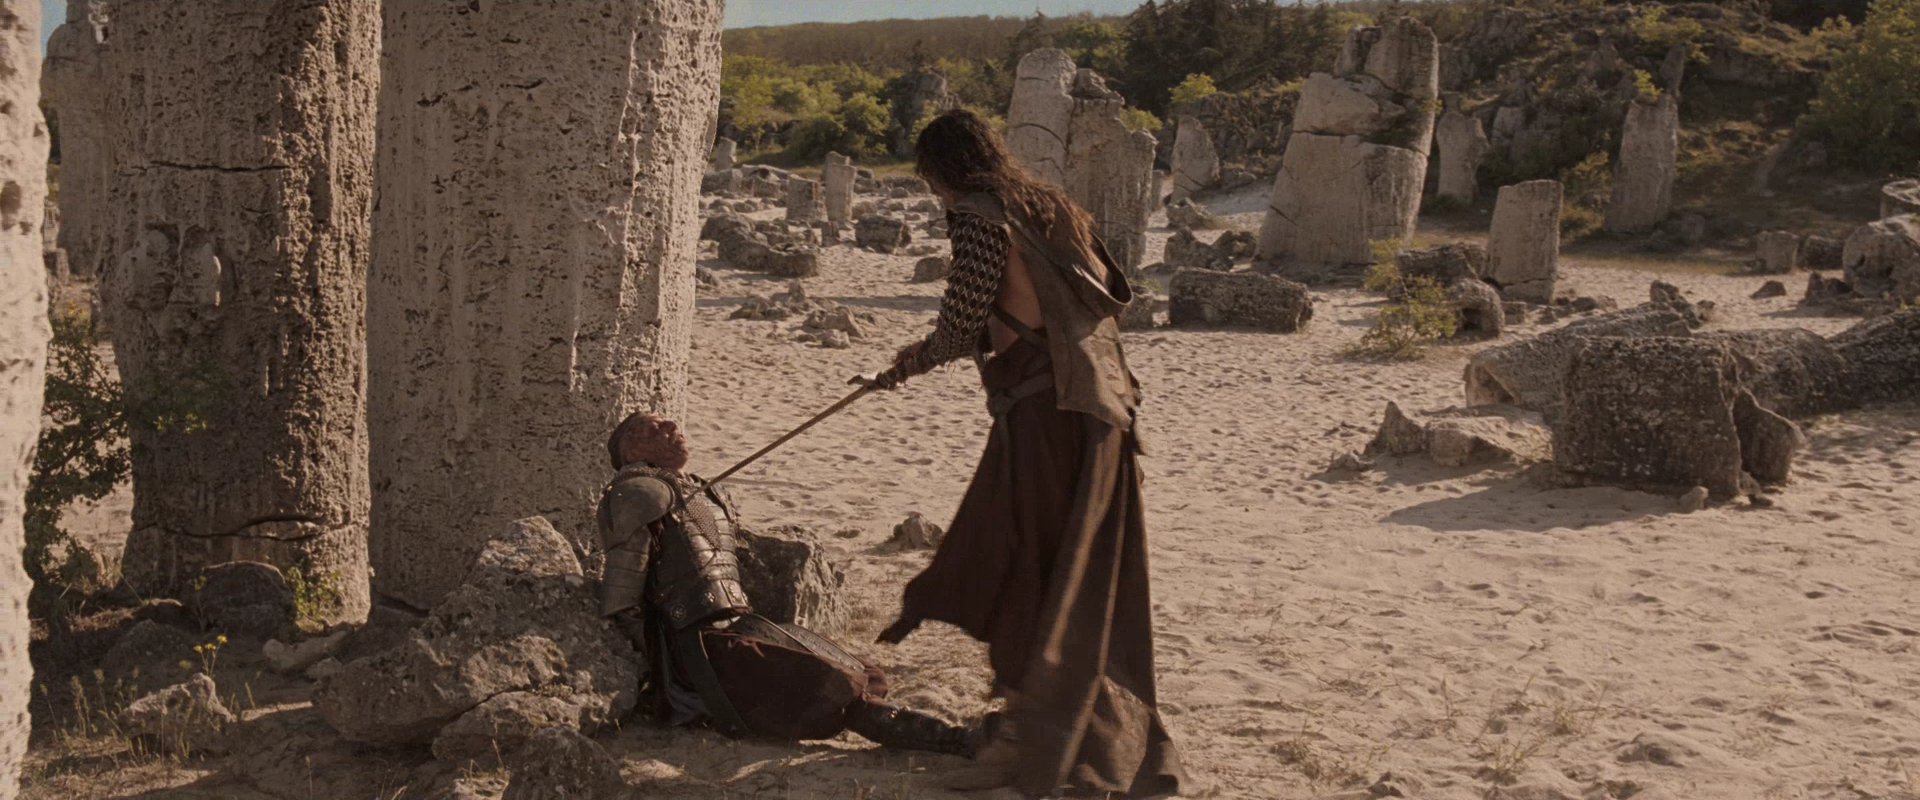
\includegraphics[width=\linewidth]{src} }
		\centerline{\scriptsize{(c) Source left view}}\medskip
	\end{minipage}%
	\hfill
	\begin{minipage}[b]{0.49\linewidth}
		\centering
		\centerline{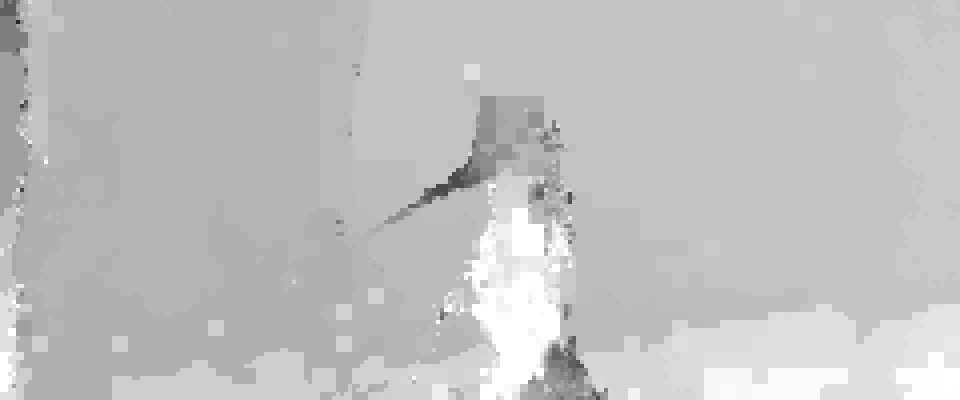
\includegraphics[width=\linewidth]{merged} }
		\centerline{\scriptsize{(d) Overall motion-strength map}}\medskip
	\end{minipage}
	\begin{minipage}[b]{\linewidth}
	\caption{Example maps of horizontal~(a) and vertical~(b) motion extracted
        using a block-based motion-estimation algorithm~\cite{simonyan2008fast} for the source frame~(c).
        The results  are combined into an overall motion-strength map~(d).}
    \label{fig:merged}
    \end{minipage}
\end{figure}

\begin{figure}[!h]
	\begin{minipage}[b]{1.0\linewidth}
		\centering
		\centerline{ 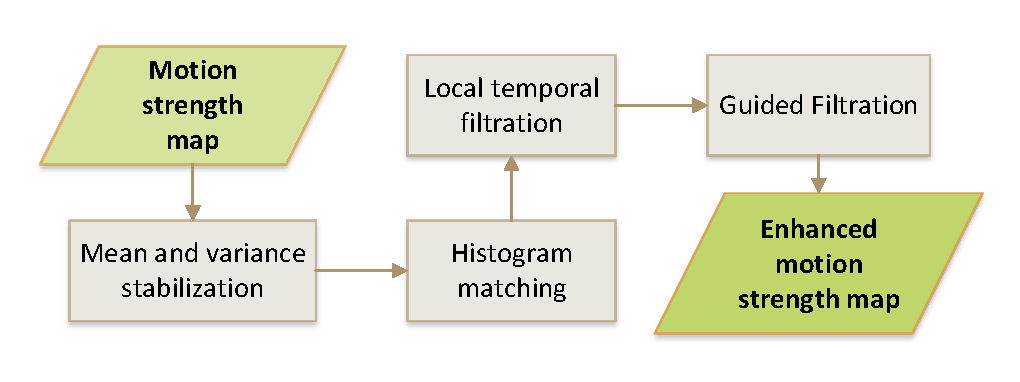
\includegraphics[width=\textwidth]{dfm_pipeline.pdf} }
	\end{minipage}
    \caption{Pipeline of spatio-temporal filtering. This approach enables us to enhance the rough
        motion-intensity map that we obtain from the motion-estimation algorithm.}
	\label{fig:dfm}
\end{figure}


Элементы карты амплитуды движения $M$ высчитываются, как величины в поле векторов 
движения (см. Рис.~\ref{fig:merged}~(а) и (б)). Затем, для увеличения временной стабильности
полученной карты интенсивности, применяются последовательно временные и пространственные 
фильтрации, составляющие конвейер алгоритмов, изображенный на Рис.~\ref{fig:dfm}.

Процесс улучшения начинается с применения линейного преобразования к карте амплитуды движения;
данное преобразование выставляет минимальное значение элементов в карте равным 0, а максимальное --- 1
(также известное, как автоматическая тоновая коррекция). Рис.~\ref{fig:merged}~(г) демонстрирует
промежуточный результат для этого шага. Из-за непостоянства скоростей движения камеры 
и объектов в сцене, а также из-за ошибок в поле векторов движения, результирующие карты 
интенсивности заметно мерцают. Для сокращения влияния данного эффекта, происходит 
выравнивание среднего и дисперсии интенсивности каждого кадра на величину, равную 
соответствующим значениям, рассчитанным за последние $n$ кадров (в экспериментах использовалось $n = 10$):
\begin{equation}
M_{i}^{'k} = \frac{\mathsf{Std}_{k-n}^{k-1}}{\mathsf{Std}\left[M^k\right]} \left( M_i^k - \mathsf{E}\left[M^k\right]\right) + \mathsf{E}_{k-n}^{k-1}
\end{equation}
Здесь, $\mathsf{E}$ и $\mathsf{Std}$ --- математическое ожидание и стандартное отклонение, соответственно; 
$M^k_i$ --- пиксель $i$ карты амплитуды движения для кадра $k$; $\mathsf{E}_{k-n}^{k-1}$ и 
$\mathsf{Std}_{k-n}^{k-1}$ --- математическое ожидание и стандартное отклонение во времени, соответственно. 
Эти значения получаются по следующим формулам:
\begin{equation}
\mathsf{E}_{k-n}^{k-1} =  \frac{1}{\#} \sum_{i}\left(\frac{1}{n}\sum_{p=k-n}^{k-1}M_i^p\right)
\label{fm:temp_mean}
\end{equation}
\begin{equation}
\mathsf{Std}_{k-n}^{k-1} = \sqrt{\frac{1}{\# - 1} \sum_{i}\left(\frac{1}{n}\sum_{p=k-n}^{k-1}M_i^p - \mathsf{E}_{k-n}^{k-1}\right)^2}
\label{fm:temp_std}
\end{equation}

\begin{figure}[!h]
	\begin{minipage}[b]{0.49\linewidth}
		\centering
		\centerline{ 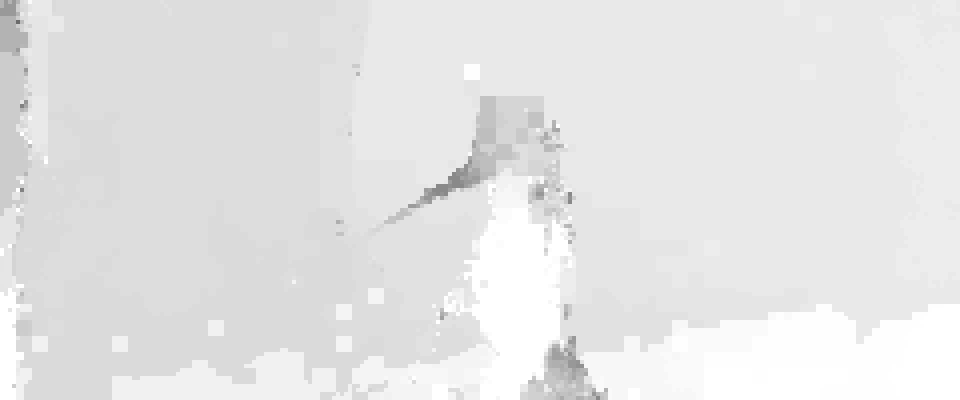
\includegraphics[width=\linewidth]{mean_and_variance} }
		\centerline{(а) Результат стабилизации}
		\centerline{среднего и дисперсии}\medskip
	\end{minipage}%
	\hfill
	\begin{minipage}[b]{0.49\linewidth}
		\centering
		\centerline{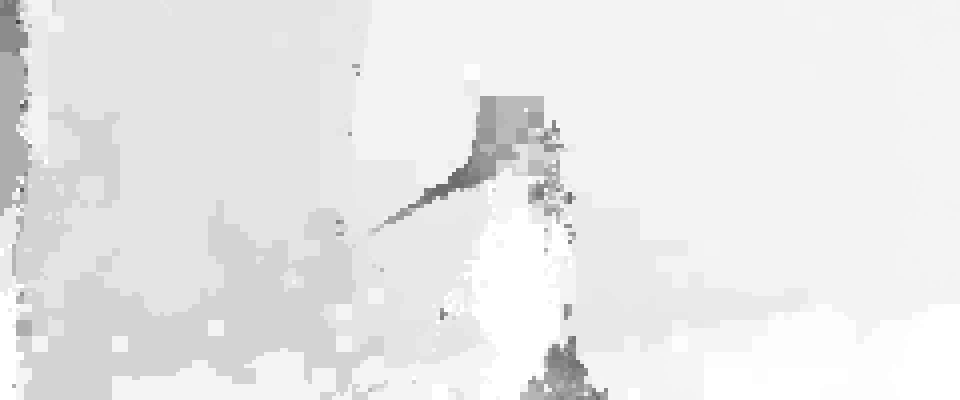
\includegraphics[width=\linewidth]{histogram_matching} }
		\centerline{(б) Результат сопоставления}
		\centerline{гистограмм}\medskip
	\end{minipage}
	\hfill
	\begin{minipage}[b]{0.49\linewidth}
		\centering
		\centerline{ 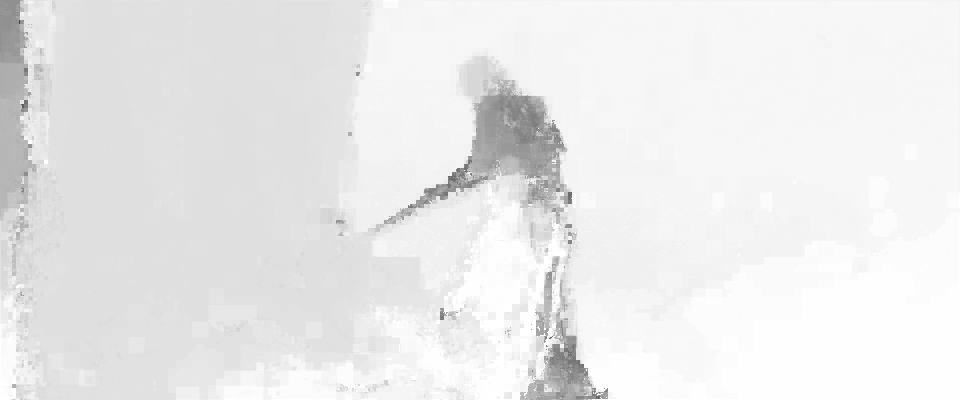
\includegraphics[width=\linewidth]{stabilization} }
		\centerline{(в) Результат временной}
		\centerline{фильтрации}\medskip
	\end{minipage}%
	\hfill
	\begin{minipage}[b]{0.49\linewidth}
		\centering
		\centerline{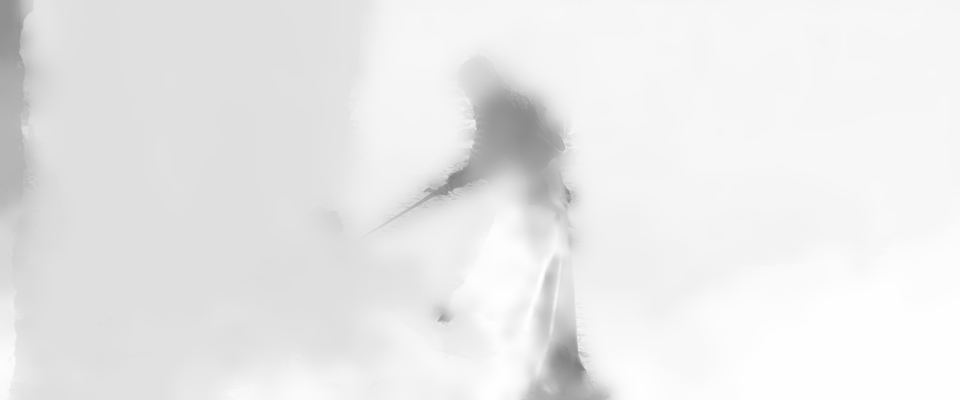
\includegraphics[width=\linewidth]{guided_filtration} }
		\centerline{(г) Результат применения}
		\centerline{Guided filter}\medskip
	\end{minipage}
	\begin{minipage}[b]{\linewidth}
    \caption{ Примеры, иллюстрирующие каждый промежуточный этап конвейера
    	просранственно-временных фильтраций из Рис.~\ref{fig:dfm}.}
    \label{fig:filtered}
    \end{minipage}
\end{figure}


В равенствах (\ref{fm:temp_mean}) и (\ref{fm:temp_std}) $\#$ обозначает число пикселей в кадре.
На Рис.~\ref{fig:filtered}~(а) изображен промежуточный результат после этого шага. В качестве
глобального преобразования применяется сопоставление гистограмм~\cite{fecker2007time}
к последовательности карт амплитуды движения. Данное преобразование сдвигает 
гистограмму для каждого кадра так, что она соответствует средней гистограмме 
для предыдущих  $n$ кадров. Пример можно увидеть на Рис.~\ref{fig:filtered}~(б).

Для того, чтобы убрать локальные мерцания, возникающие после глобальных преобразований,
используется метод временной стабилизации, описанный в~\cite{matyunin2011temporal} 
(см. пример на Рис.~\ref{fig:filtered}~(в)).

На последнем шаге для согласования границ карты амплитуды движения с границами 
исходного ракурса кадра, а также для заполнения областей с низким доверием,
используется guided filter~\cite{he2013guided}, на вход которому в качестве
направляющего изображения передается исходный ракурс. Рис.~\ref{fig:filtered}~(г)
демонстрирует пример финальной карты амплитуды движения.

\subsection{Карта диспаратности}

\begin{figure}[t]
	\begin{minipage}[b]{0.49\linewidth}
		\centering
		\centerline{ 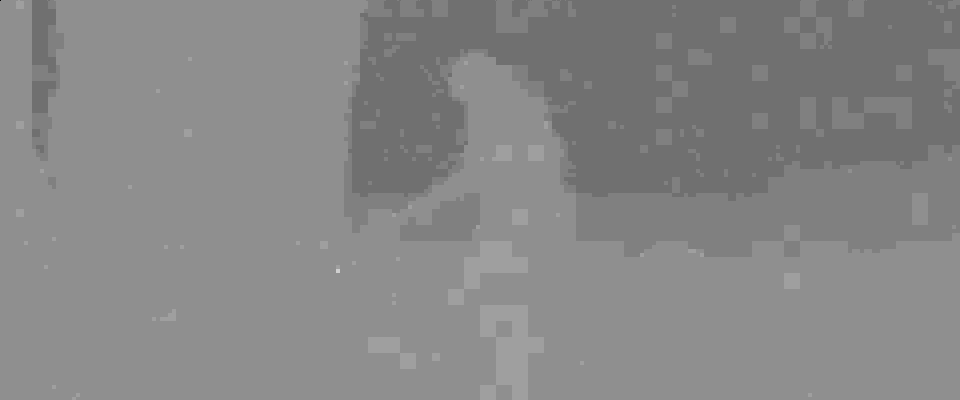
\includegraphics[width=\textwidth]{disp} }
		\centerline{\scriptsize{(a) Estimated disparity map }}\medskip
	\end{minipage}
	\hfill
	\begin{minipage}[b]{0.49\linewidth}
		\centering
		\centerline{
\includegraphics[width=\textwidth]{wmf} }
		\centerline{\scriptsize{(b) Enhanced disparity map}}\medskip
	\end{minipage}
	\begin{minipage}[b]{1\linewidth}
		\centering
		\centerline{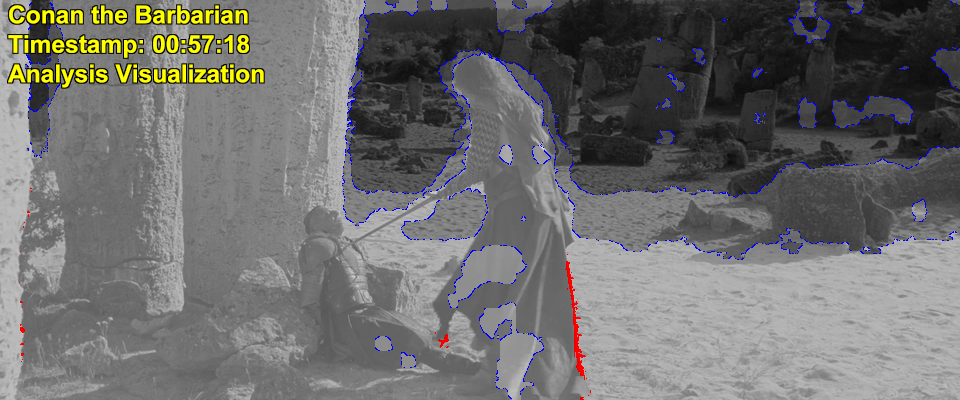
\includegraphics[width=\textwidth]{visualization} }
		\centerline{\scriptsize{(c) Visualization of final result }}
	\end{minipage}
    \caption{Examples of a disparity map before~(a) and after~(b) weighted-median
        filtering. The resulting visualization~(c) that we offer to content
        creators is a disparity map overlaid on the source frame. We use blue to mark
        the disparity edges and red to mark any inconsistencies
        between motion- and disparity-map edges.}
	\label{fig:disp}
\end{figure}


Существуют ситуации, когда нет возможности оценить используемые карты глубины напрямую. 
В таких случаях оценивается карта диспаратности с помощью блочного алгоритма сопоставления. 
Для увеличения качества карты используется быстрая версия фильтрации взвешенной медианы,
описанной в~\cite{zhang2014100+}. Данная фильтрация улучшает контуры объектов и
устраняет посторонние границы в местах, которые отвечают плавным переходам по глубине.
Пример оцененной карты перед и после применения фильтрации можно найти на Рис.~\ref{fig:disp}~(а) и (б).

\subsection{Сопоставление границ}

\begin{figure}[t]
	\begin{minipage}[b]{0.49\linewidth}
		\centering
		\centerline{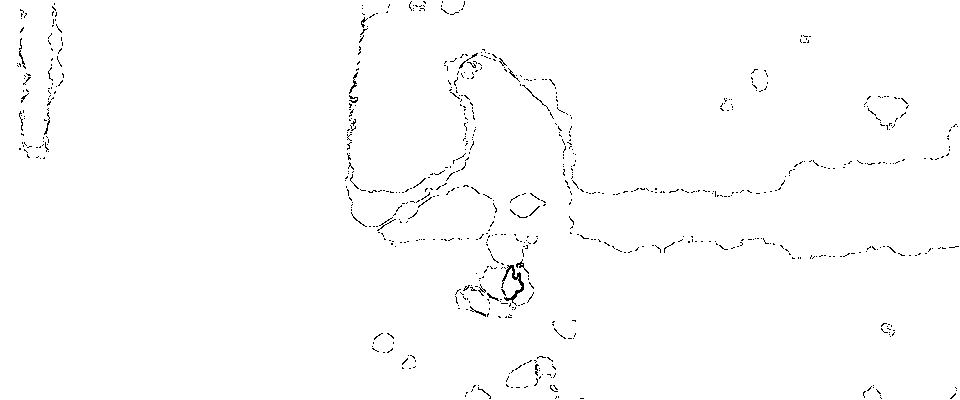
\includegraphics[width=\textwidth]{disparity_contours} }
		\centerline{(а) Границы, извлеченные}
		\centerline{из карты диспаратности}\medskip
	\end{minipage}
	\begin{minipage}[b]{0.49\linewidth}
		\centering
		\centerline{ 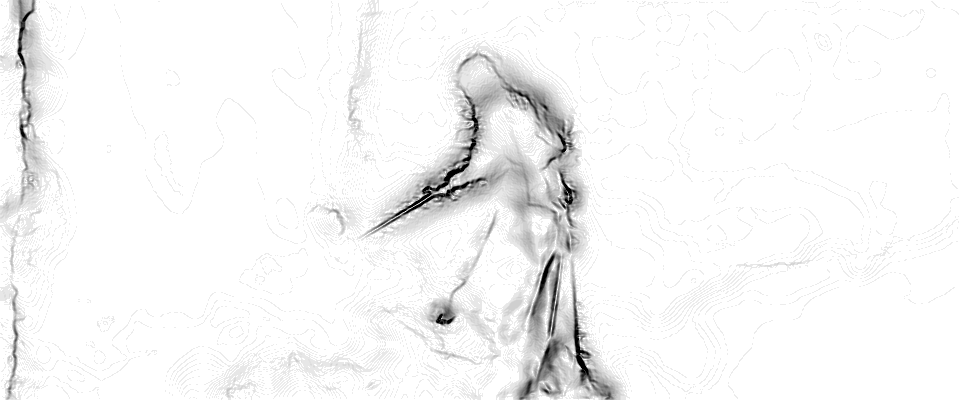
\includegraphics[width=\textwidth]{drop_contours} }
		\centerline{(б) Границы, извлеченные}
		\centerline{из карты амплитуды движения}\medskip
	\end{minipage}
	\hfill
	\begin{minipage}[b]{0.49\linewidth}
		\centering
		\centerline{ 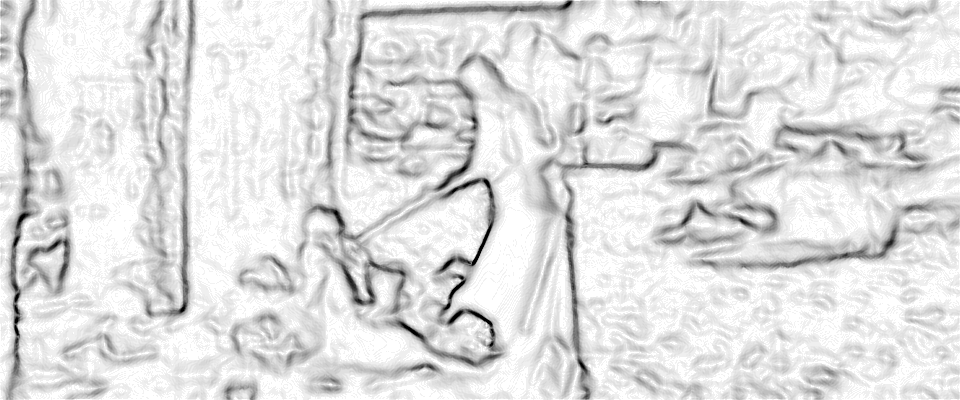
\includegraphics[width=\textwidth]{src_contours} }
		\centerline{(в) Границы, извлеченные}
		\centerline{из исходного кадра}\medskip
	\end{minipage}
	\hfill
	\begin{minipage}[b]{0.49\linewidth}
		\centering
		\centerline{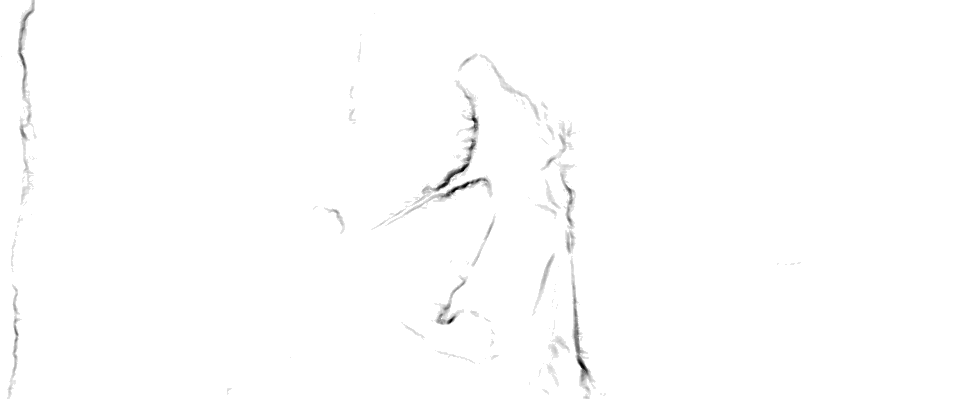
\includegraphics[width=\textwidth]{dfm_contours} }
		\centerline{(г) Пересечение границ}\medskip
		\centerline{движения~(б) и исходных~(в)}\medskip
	\end{minipage}
	\begin{minipage}[b]{\linewidth}
    \caption{Границы, извлеченные из карты диспаратности~(а), улучшенной карты
    	амплитуды движения~(б), и исходного кадра после применения фильтрации,
    	сохраняющей контуры объектов~(в). Пересечение границ карты интенсивности
    	движения и исходного кадра изображено на~(г).}
    \label{fig:edges}
    \end{minipage}
\end{figure}


Для извлечения границ применяется оператор Щарра~\cite{jahne1999principles} к карте
амплитуды движения после фильтрации и к карте глубины. Результирующие карты границ
изображены на Рис.~\ref{fig:edges}~(а) и (б). Так как карта интенсивности движения
содержит размытые границы, являющие следствием применения guided filter, используется
информация с исходного RGB кадра для их уточнения. Однако простое пересечение не даст
должной точности результата, так как исходный кадр содержит множество посторонних текстурных
границ. Для устранения большей части <<шумных>> границ применяется фильтрация
с учетом контуров объектов~\cite{zhang2014rolling} к исходному кадру, а границы извлекаются 
из уже отфильтрованного изображения (см. Рис.~\ref{fig:edges}~(г)).

В конце вычисляется пересечение извлеченных границ из карты амплитуды движения ($M$) 
и исходного кадра после фильтрации  ($I$) следующим образом:
\begin{equation}
M_i^{'k} =M_i^k\max_{j  \in B_{r}(i)}(I_j^k)
\end{equation}
Здесь, $B_{r}(i)$ --- это окрестность радиуса $r = 0$ вокруг пикселя $i$. Для улучшения границ 
карты диспаратности используется схожая процедура с $r = 5$.

Для получения итоговой оценки качества производится пересечение границ улучшенной карты
амплитуды движения с границами карты диспаратности методом, основанным на алгоритме
distance transform. Для каждого пикселя границы в карте интенсивности движения итеративно
вычисляется значение расстояния:
\begin{equation}
\begin{split}
M_i^{k,0} &= M_i^k, \\
M_i^{k,t} &= M_i^{k,t-1} - \max_{j \in B_t(i)}w(i,j)\frac{\left(\vec{M}_i^{k,t-1}, \vec{D}_j  \right)}{\lVert\vec{D}_j\rVert}
\end{split}
\end{equation}
В этом выражении $w(i,j)$  --- функция веса, зависящая от расстояния:
\begin{equation}
w(i,j) = \exp\left(\frac{\lVert i-j \rVert^2}{2\sigma^2}\right)
\end{equation}
Здесь, $\vec{M}_i^{k,t-1}$ и $\vec{D}_j$ --- карты границ амплитуды движения и диспаратности, 
извлеченные с помощью оператора Щарра. Итоговая карта содержит только те границы,
которые присутствуют на карте движения, но отсутствуют на карте глубины. Такие границы,
вероятно, принадлежат объектам, частично или полностью отсутствующим на карте глубины.
Пример итогового результат можно найти на Рис.~\ref{fig:disp}~(в) (потерянные границы 
по мнению алгоритма, изображены красными линиями).

\newpage
\section{Экспериментальная оценка}

\subsection{Валидация алгоритма}

\begin{table}[!h]
	\centering
	\begin{tabular}[width=\textwidth]{lcc}
		\toprule
		Film 										&  True positive  & False positive  		 \\\toprule
		Clash of the Titans 			& 5 								 & 5 						   \\\midrule
		Conan the Barbarian 		& 4 								 & 12 						  \\\midrule
		Star Trek Into Darkness   & 1 								    & 7 						  \\\midrule
		Harry Potter and  				&  									   &  							   \\
		the Deathly Hallows: 		 & 4 								   & 7						     \\
		Part 2 									  & 									  & 							 \\\midrule
		The Avengers 					 & 7 									& 0 						 \\\bottomrule
	\end{tabular}
    \caption{Number of true- and false-positive detections by initial algorithm for the validation data set.}
	\label{tab:testsample}
\end{table}


Алгоритм, реализующий метод, описанный в предыдущем разделе, был использован 
для определения отношения ложных и истинных срабатываний на множестве из 5 фильмов.
Для создания валидационного множества, сцены, на которых алгоритм выдал высокие значения, 
были вручную классифицированны как истинно и ложно положительные. 
Итоговый набор сцен состоял из 21 истинно положительной сцены 
и 31 ложно положительной (см. Таблицу~\ref{tab:testsample}).

\begin{figure}[!h]
	\begin{minipage}[b]{0.49\linewidth}
		\centering
		\centerline{ 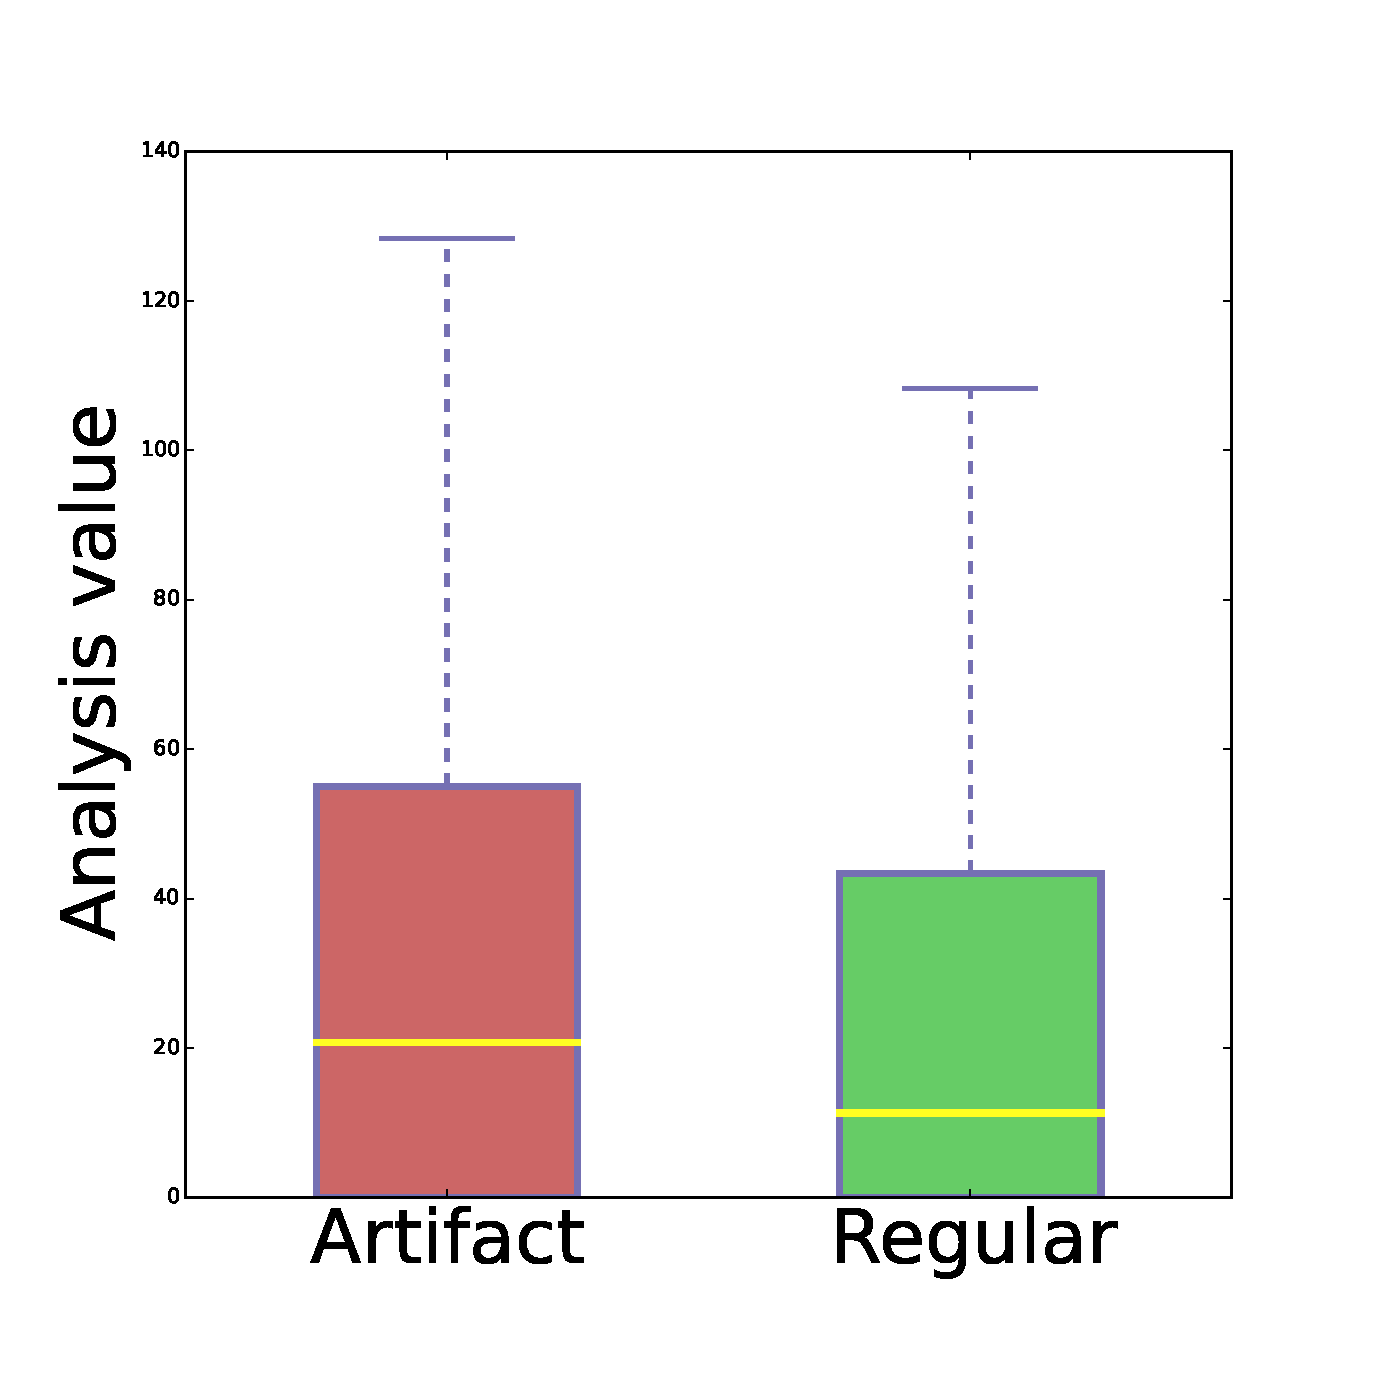
\includegraphics[width=\textwidth]{v1_test} }
		\centerline{\scriptsize{(a) Scores computed using}}
		\centerline{\scriptsize{initial algorithm}}\medskip
	\end{minipage}
	\hfill
	\begin{minipage}[b]{0.49\linewidth}
		\centering
		\centerline{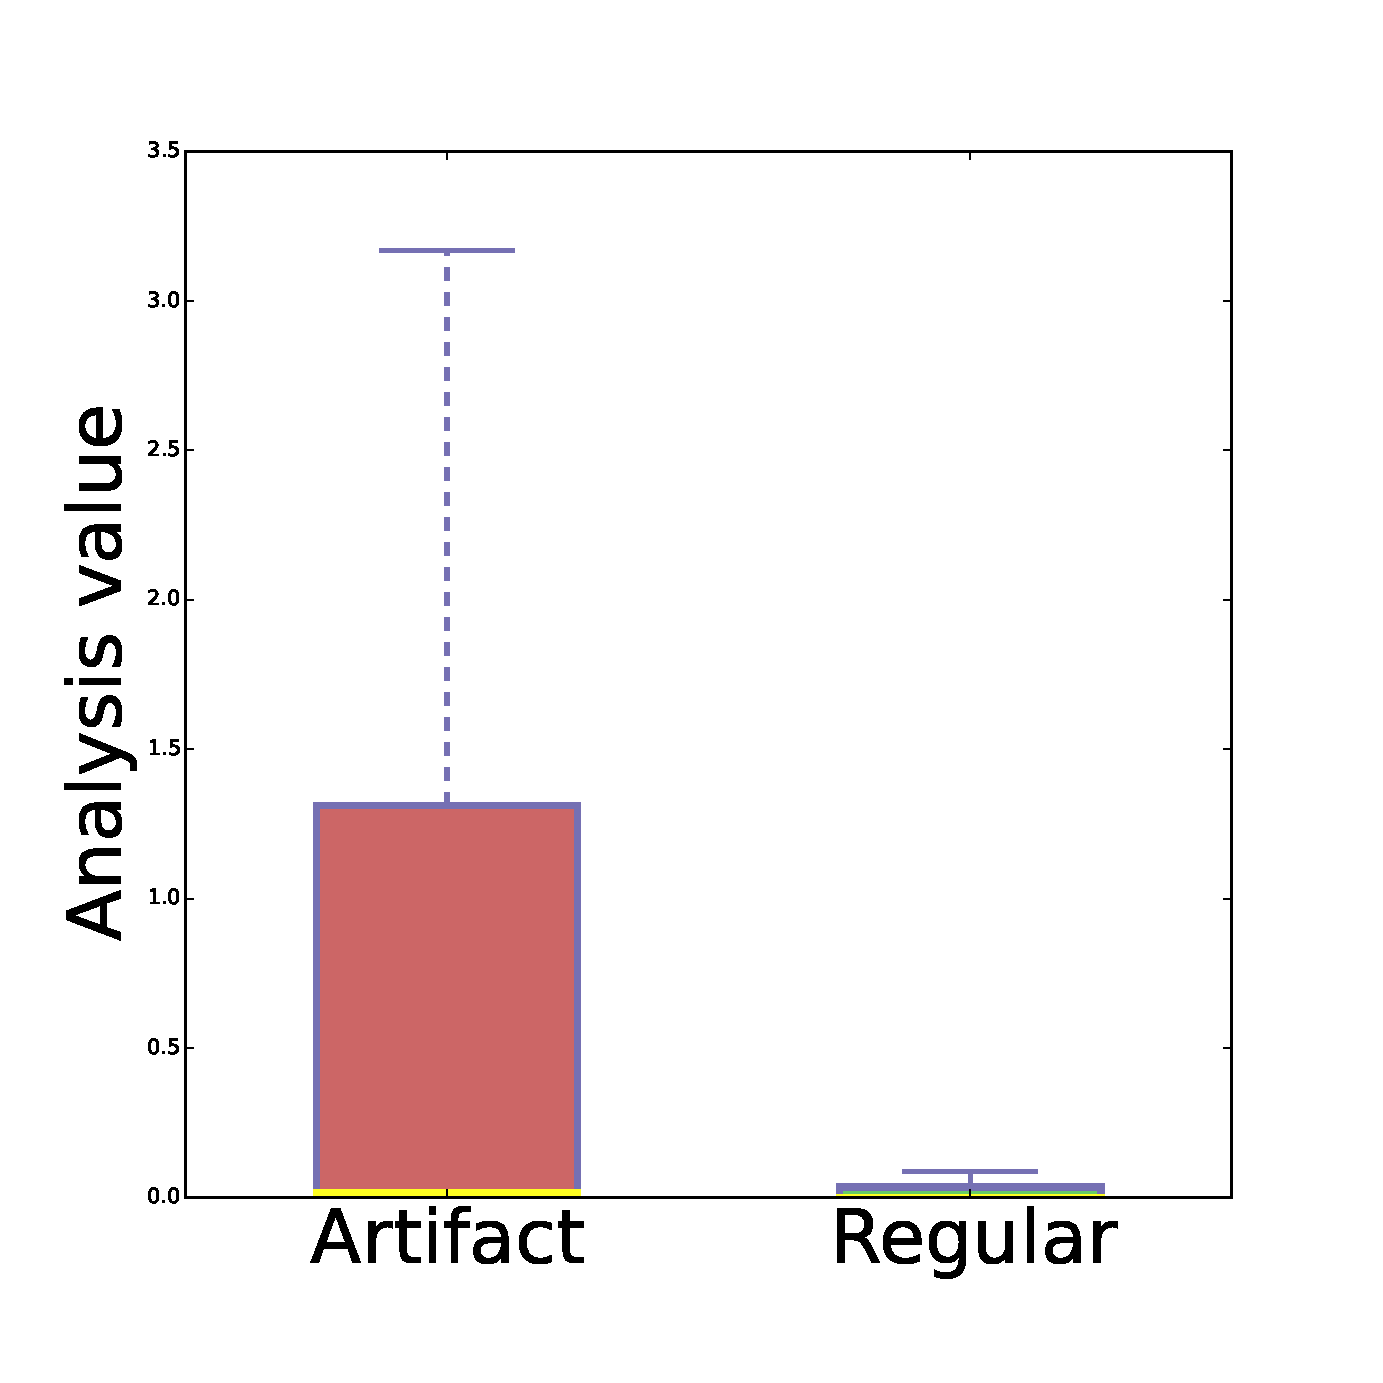
\includegraphics[width=\textwidth]{v2_test} }
		\centerline{\scriptsize{(b) Scores computed using}}
		\centerline{\scriptsize{modified algorithm}}\medskip
	\end{minipage}
    \caption{Mean scores of the initial algorithm~(a) for true- and false-positive
        scenes, as well as mean scores computed for the same scenes using an algorithm modified
        to exclude RGB uniform regions~(b).}
	\label{fig:textureless}
\end{figure}


Как показала классификация, основным источником ошибок второго рода оказались
объекты, находящиеся перед монотонным фоном (например, небо). Так как блочный
алгоритм оценки диспаратности выдает неточности в малотекстурированных 
областях, предлагаемый метод не способен найти разницу между диспаратностью
объекта переднего плана и фона, даже если объект присутствует на карте глубины.
Более того, зрительная система человека терпимо относится к отсутствию различия
по глубине в малотекстурированных областях. Таким образом, разумным подходом
сокращения количества ложных срабатываний  является исключение из рассмотрения
алгоритма любых объектов, возникающих перед монотонным фоном. Это достигается
с помощью добавления весового множителя к значениям итоговой карты пересечения,
который будет равен цветовой дисперсии в некоторой окрестности для
каждого пикселя исходного кадра. Рис.~\ref{fig:textureless} демонстрирует
сравнение оценок, вычисленных обычным подходом и модифицированным 
для сцен из валидационного множества. Модифицированной версии алгоритма удается
отличить сцены с артефактами от сцен, ошибочно оцененных простой версией.

\subsection{Анализ полнометражных фильмов}

\begin{figure}[!h]
	\begin{minipage}[b]{1.0\linewidth}
		\centering
		\centerline{ 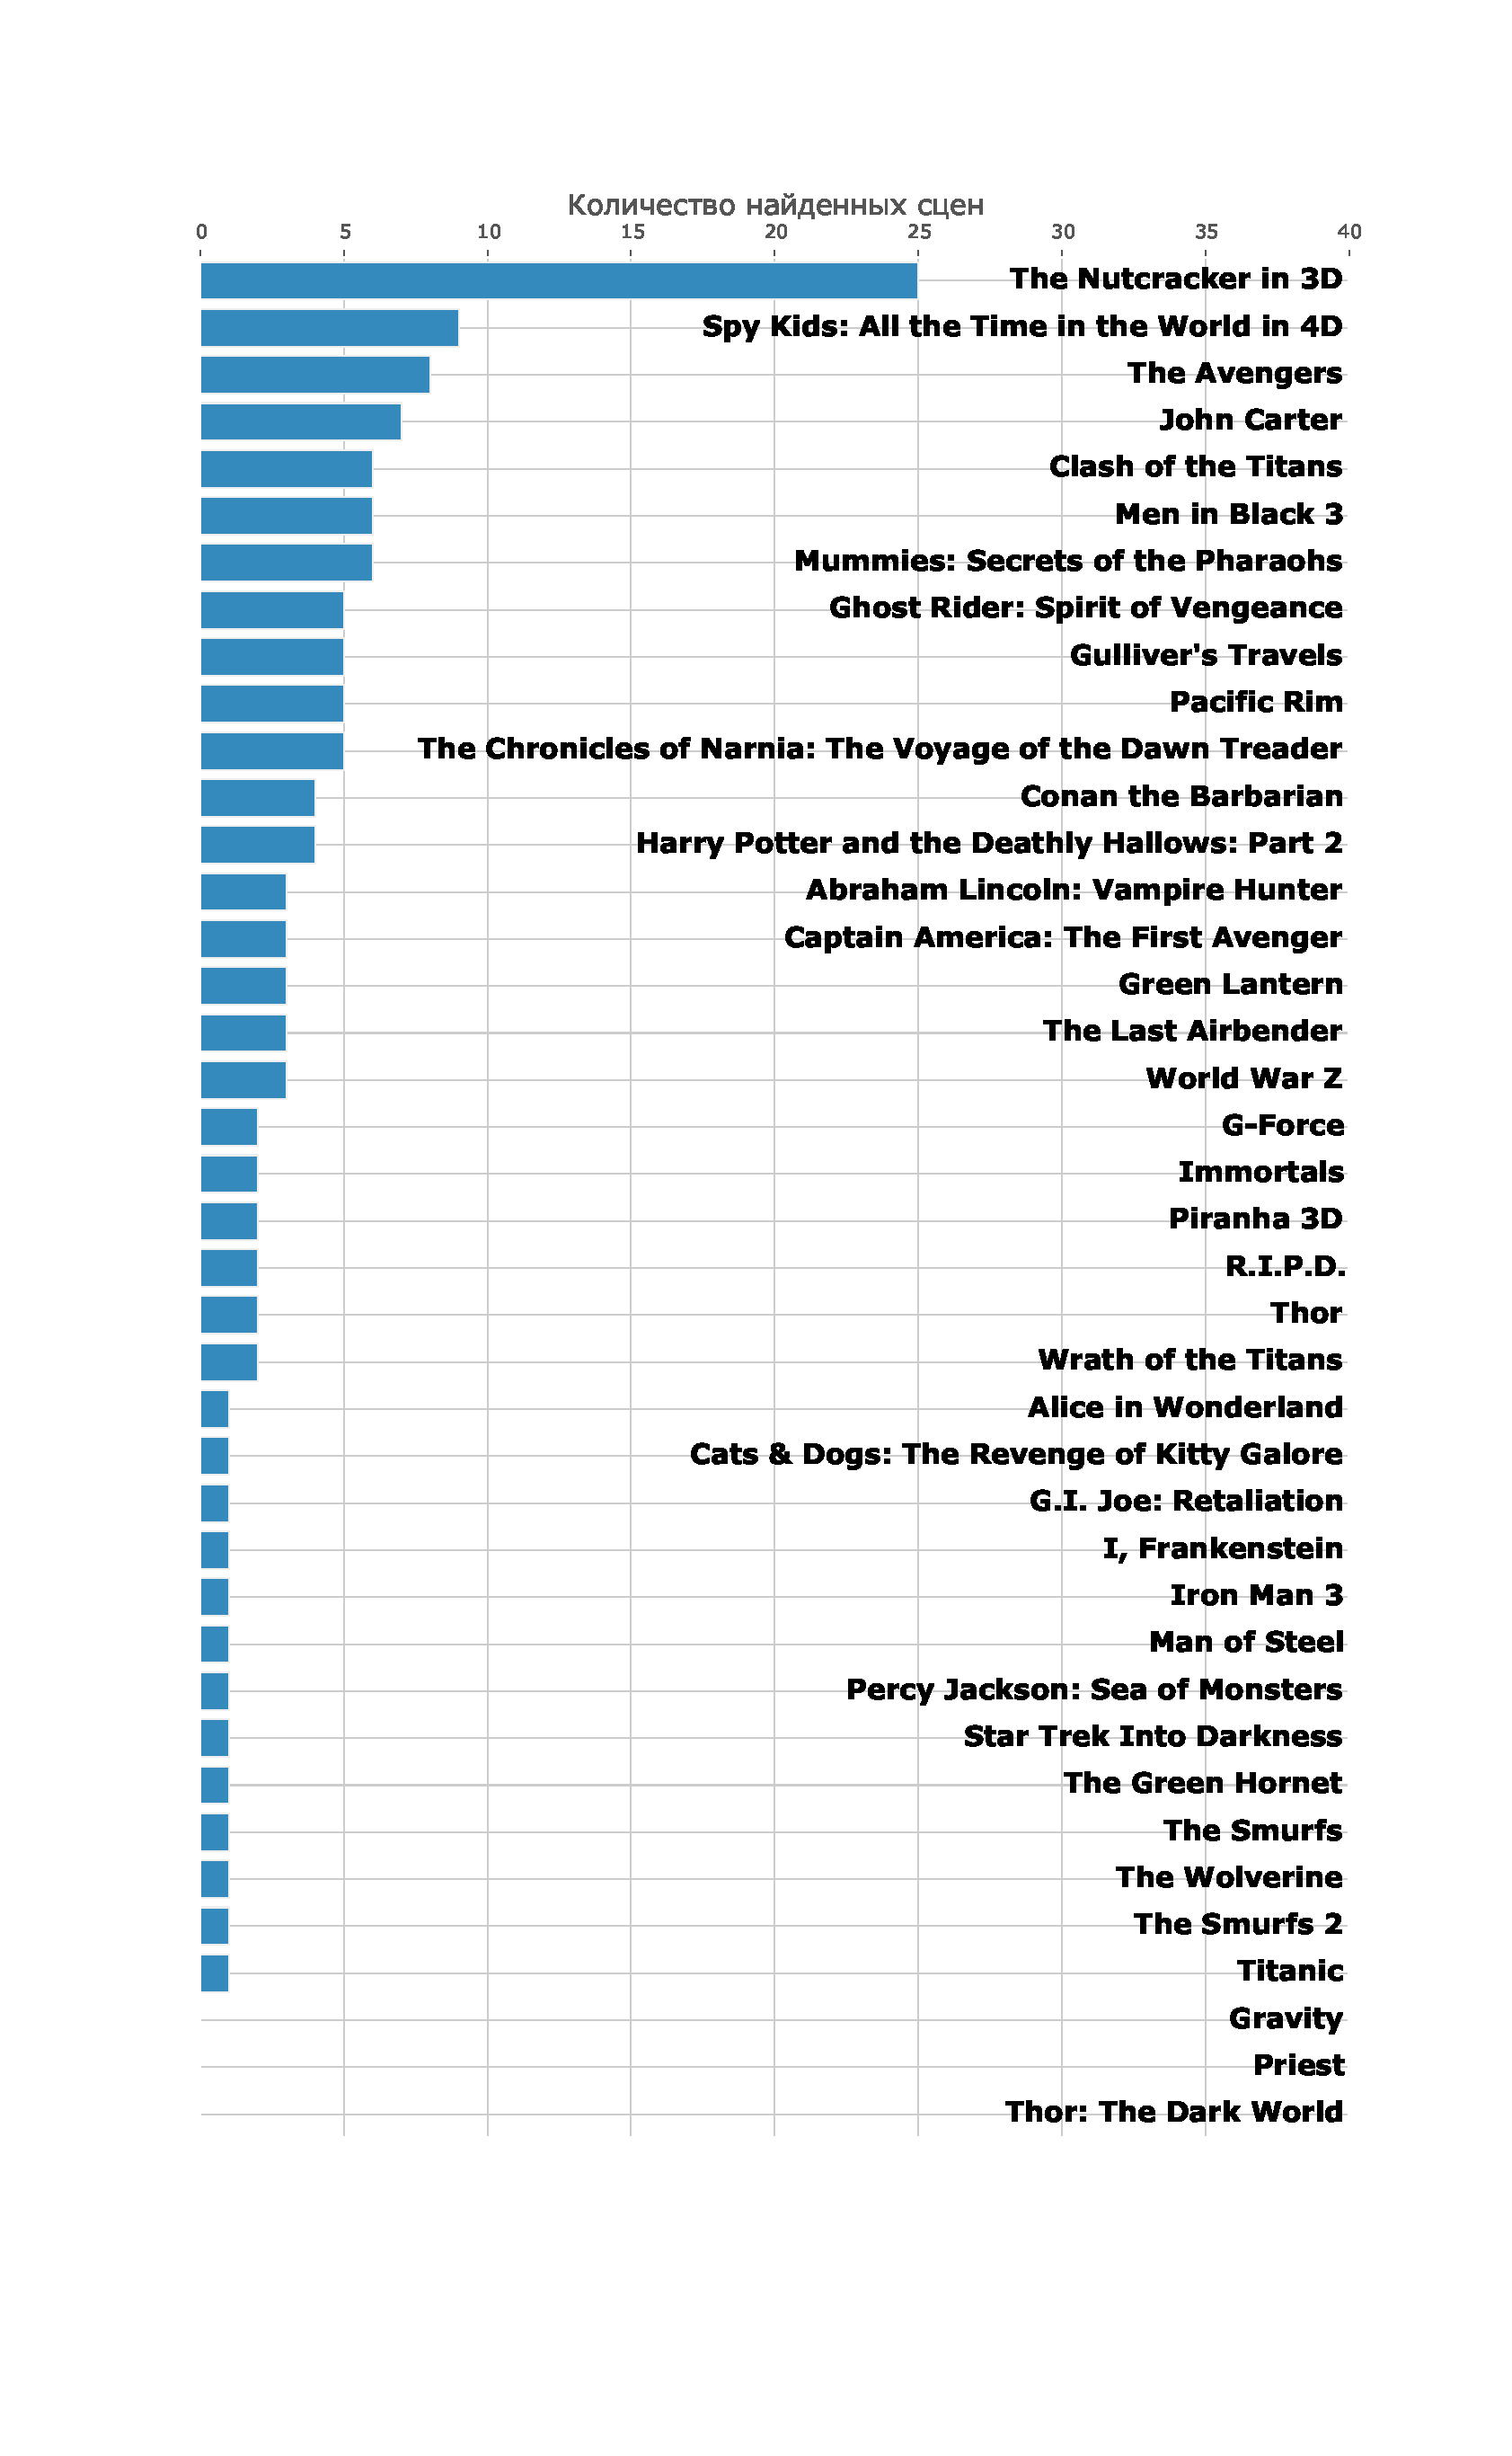
\includegraphics[width=0.82\textwidth, trim= 50 150 50 60, clip]{all_films_rus} }
	\end{minipage}
    \caption{Количество сцен с заметными артифактами, найденных 
    	в процессе анализа полнометражных фильмов.}
	\label{fig:results}
\end{figure}


После модификации алгоритм был запущен на 39 стереоскопических полнометражных
фильмах с конвертированным стерео. В итоге было найдено 125 проблемных сцен. 
На Рис.~\ref{fig:results} изображен график распределения количества сцен, 
найденных в каждом из анализируемых фильмов.

\begin{figure}[!h]
	\begin{minipage}[b]{1.0\linewidth}
		\centering
		\centerline{ 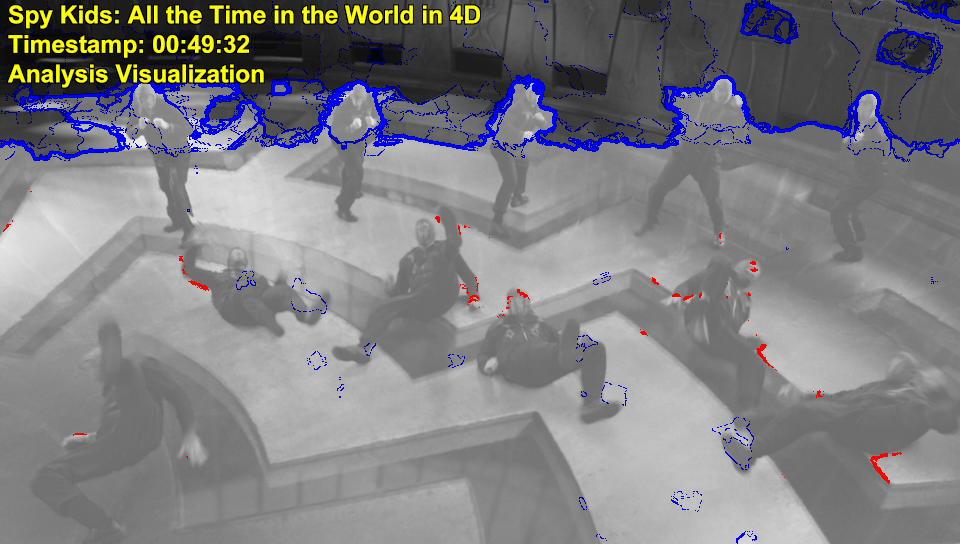
\includegraphics[width=0.8\textwidth]{example_spy} }
	\end{minipage}
	\begin{minipage}[b]{1.0\linewidth}
		\centering
		\centerline{ 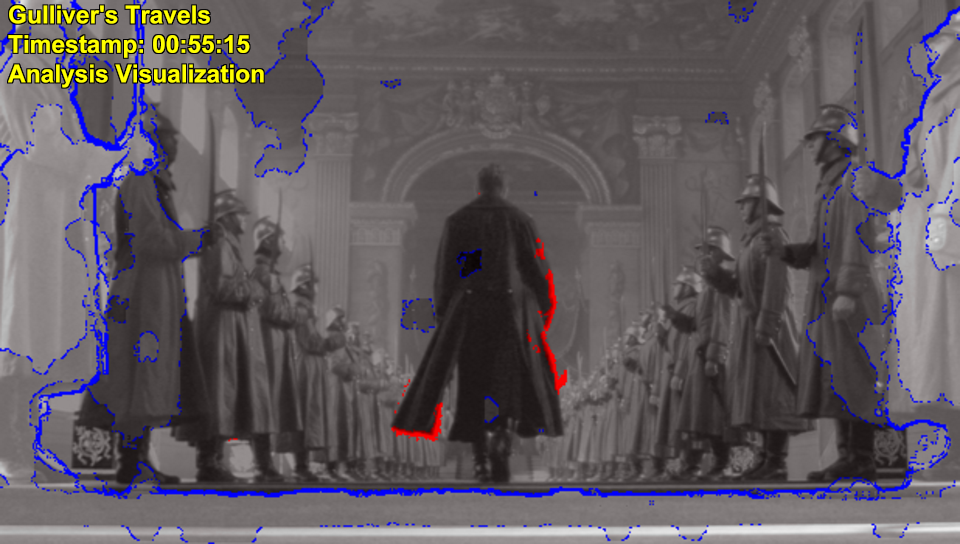
\includegraphics[width=0.8\textwidth]{example_gulliver} }
	\end{minipage}
    \caption{Пример результатов срабатвания алгоритма. В данных сценах
    	объекты переднего плана <<слиты>> с фоном. Для наглядности
    	поверх исходного кадра изображены карта диспаратности, границы
    	карты диспаратности (синие), и границы объектов, которые алгоритм посчитал
    	потерянными (красные).}
	\label{fig:res_example}
\end{figure}


\newpage
\newpage
\newpage
\clearpage
\section{Программная реализация}

Алгоритм был реализован в виде подключаемого DLL-модуля к автоматизированной 
системе оценки качества стереокино в рамках проекта VQMT3D 
(Video Quality Measurement Tool 3D). Язык реализации --- C++. Среда разработки --- 
Microsoft Visual Studio 2013. Применялась библиотека OpenCV, а также программная 
реализация алгоритма определения движения MSU Motion Estimation. 
Реализация алгоритма насчитывает 1000 строк. 

Для автоматизации прогонов алгоритма на тестовых наборах, построения графиков, 
извлечения найденных сцен из фильмов и генерации визуализаций были разработаны 
скрипты на языках Python и Javascript, общим объёмом в 1000 строк. 

Для анализа качества стереофильмов данный алгоритм использовался в составе 
распределённой автоматизированной системы проекта VQMT3D. Всего в анализе было 
задействовано около 10 машин, каждая из которых обсчитывала определённые сцены из фильмов.

В процессе работы в составе системы модуль получает на вход кадры ракурсов. 
По окончании обработки кадра в выходной файл записывается значение оценки. 
Среднее время работы предложенного метода анализа при обработке 
видеопоследовательности с разрешением $960\times540$ около 3.5~секунд
на машине с характеристиками: 2.67 GHz Intel Core i7, 24 GB of RAM. 

\begin{figure}[!h]
	\begin{minipage}[b]{1.0\linewidth}
		\centering
		\centerline{ 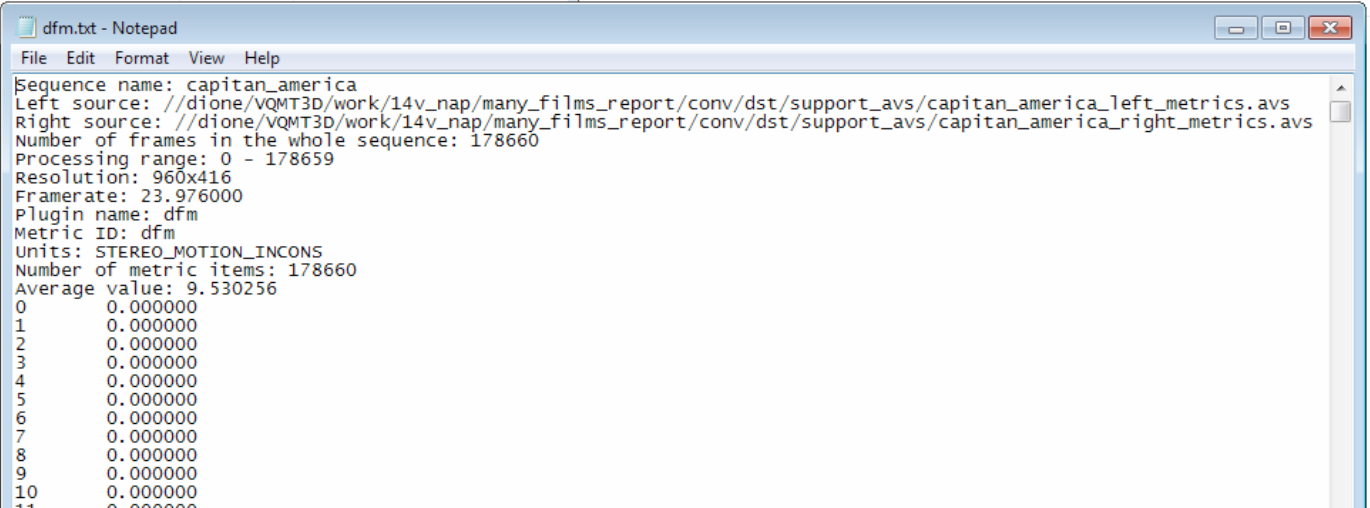
\includegraphics[width=0.7\textwidth]{shot} }
	\end{minipage}
    \caption{Пример файла результатов работы модуля оценки качества 
    	конвертированного стереовидео для системы обсчёта VQMT3D.}
	\label{fig:system_example}
\end{figure}


\newpage
\section{Заключение}

\subsection{Результаты работы}

В данной выпускной квалификационной работе был 
предложен метод оценки качества карт глубины,
используемых при конвертации стереоскопического видео. Метод находит объекты
переднего плана, которые оказались <<слиты>> с фоном на карте глубины,
что позволит создателям конвертированных фильмов найти и исправить данную проблему.
Была рассмотрена предметная область, в частности, аналоги алгоритмов, которые легли
в основу предлагаемого метода.

Качество метода было продемонстрировано с помощью валидационного множества сцен, 
состоящего из 5 фильмов. Количество ложных срабатываний было уменьшено
с помощью исключения из анализа малотекстурированных областей. Использование
быстрого извлечения глубины из движения позволило проанализировать 39
полнометражных конвертированных стереоскопических фильмов и найти
125 сцен со значительными артефактами, которые могут вызвать визуальный
дискомфорт зрителя.

\subsection{Публикации и гранты}

По теме данной работы были сделаны следующие публикации:

\begin{itemize}
	\item Dolganov S. et al. Detection of stuck-to-background objects in converted S3D movies // 3D Imaging (IC3D), 2015 International Conference on. – IEEE, 2015. – С. 1-6.
	\item Долганов С. В. <<Метод поиска несоответствий границ объектов между результатом 2D-3D конвертации и используемыми картами глубины>> // XXIII Международная конференция студентов, аспирантов и молодых ученых <<Ломоносов-2016>>, стр. 11-13.
\end{itemize}

Также работа была частично поддержана грантами У.М.Н.И.К. и РФФИ № 15-01-08632-а.

\newpage
\addcontentsline{toc}{section}{Список литературы}
\bibliographystyle{gost2008}
\bibliography{dipbib}

\end{document} 